\documentclass[conference]{IEEEtran}
\IEEEoverridecommandlockouts
\usepackage{cite}
\usepackage{amsmath,amssymb,amsfonts}
\usepackage{algorithmic}
\usepackage{graphicx}
\usepackage{mathptmx}   % force Times for text and math
\usepackage{textcomp}
\usepackage{xcolor}
\def\BibTeX{{\rm B\kern-.05em{\sc i\kern-.025em b}\kern-.08em
    T\kern-.1667em\lower.7ex\hbox{E}\kern-.125emX}}
\begin{document}

\title{Before the Docks Run Dry: Forecasting Dublin Bikes Availability for Proactive Rebalancing with Open Urban Data}

\author{\IEEEauthorblockN{Himanshu Devendrasing Rajput}
\IEEEauthorblockA{\textit{MSc in Data Analytics, School of Computing} \\
\textit{National College of Ireland}\\
Dublin, Ireland \\
x24230308@student.ncirl.ie}
}

\maketitle

\begin{abstract}
Station-based bike-sharing systems fail their users in two ways: a station with no bikes blocks a pick-up, and a station with no free docks blocks a return. Operators counter this with manual rebalancing, which is expensive and often reactive. This paper presents an end-to-end, fully reproducible pipeline that predicts hourly bike availability for every station of the dublinbikes scheme using only the open Smart Dublin station-status feed. Three months of five-minute snapshots (1.86 million records, 115 stations, April to June 2026) are aggregated into 249,940 station-hours. Four models of increasing capacity, a per-station historical-mean baseline, linear regression, random forest and gradient-boosted trees, are compared under a strict temporal split: models are trained on April and May and evaluated on the unseen month of June. The best model, a random forest, attains a mean absolute error of 4.96 bikes and converts its forecasts into empty-station alerts with 78 percent precision. The predictions drive an interactive operations dashboard that classifies stations into commuter roles, ranks refill and collection priorities, and generates concrete rebalancing plans. The results show that transparent, classical machine learning on open data is sufficient to support genuinely actionable rebalancing decisions, while an honest comparison against the naive baseline exposes how much of the predictable structure lies in the weekly rhythm itself.
\end{abstract}

\begin{IEEEkeywords}
bike-sharing systems, demand forecasting, random forest, gradient boosting, open data, urban computing, temporal validation, rebalancing
\end{IEEEkeywords}

\section{Introduction}
Bike-sharing is now a fixture of European urban transport policy: it decongests streets, produces no local emissions and extends the reach of public transport. The dublinbikes scheme, operated for Dublin City Council, serves the city core with 115 docking stations. Its central operational weakness is shared by every station-based scheme: demand is strongly directional. Each weekday morning, commuters drain residential-area stations and flood workplace stations; each evening the tide reverses. A station that is empty when a rider wants a bike, or full when a rider wants to return one, represents a service failure that erodes trust in the system.

Operators mitigate this with rebalancing crews that truck bikes between stations. Rebalancing is costly, and dispatching it reactively, only after a station has already run empty, means the failure has occurred before the remedy arrives. The premise of this project is that the failure is largely predictable: if hourly availability can be forecast per station, crews can be routed \emph{before} stations run dry.

The scope of this work is deliberately end-to-end. Rather than stopping at a regression score, the project delivers (i) a cleaned, hourly station-level dataset built from the raw open feed; (ii) a defensible comparison of four forecasting approaches under leakage-free temporal evaluation; (iii) a business layer that converts numeric forecasts into empty-risk alerts with quantified precision and recall; and (iv) an interactive dashboard through which an operations team could actually consume the predictions, including an automatic rebalancing planner. All data are real, public and current, and every number reported in this paper is reproduced by a single script in the accompanying repository.

\section{Goals and Business Value}
The project pursues three concrete goals, each mapped to a measurable business outcome.

\textbf{G1: Forecast hourly availability per station.} The learning task is to predict the mean number of bikes available at a station for a given hour of day and day of week. Accuracy is reported in bikes, a unit an operations manager can reason about directly.

\textbf{G2: Convert forecasts into operational alerts.} A forecast of 11.4 bikes is not a decision. The business layer thresholds predictions into empty-risk alerts (two bikes or fewer) and full-risk alerts (two free docks or fewer), the two conditions a crew must act on. Alert quality is measured with precision, recall and F1 rather than regression error, because false alarms waste crew time while missed outages waste rider goodwill.

\textbf{G3: Make the intelligence consumable.} A Streamlit dashboard presents a city map of predicted availability for any day-hour combination, ranks stations by refill and collection urgency, classifies every station into a commuter role, and emits a concrete, downloadable rebalancing plan (which bikes to move, from where, to where, and how far the truck must travel).

The commercial logic is straightforward. With alert precision of 0.78, roughly four out of five dispatches triggered by the system target a genuine problem, and the planner batches those dispatches into an efficient route. Even marginal reductions in wasted truck runs compound daily across a fleet; the same forecasts also inform longer-horizon capacity decisions such as where additional docks would relieve chronic pressure.

\section{Related Work}
Station-level availability forecasting is an active research area. Li et al.\ established gradient-boosted regression trees for station-cluster demand prediction \cite{li2015traffic}, and Li and Zheng extended the approach to citywide usage, emphasising the dominance of calendar and meteorological regularities \cite{li2020citywide}. Yin et al.\ quantify station-level predictability directly, showing that demand uncertainty is polarised across stations, with commuter-driven stations approaching near-perfect predictability \cite{yin2023understanding}, a finding this paper's role analysis mirrors in Dublin. At the deep-learning frontier, Cho, Ham and Kim fuse public-transit usage with graph convolutional networks to sharpen peak-hour demand estimates \cite{cho2021enhancing}, and Jiang surveys the rapidly growing deep-learning literature for bike-sharing prediction, noting its appetite for large training data and its limited interpretability \cite{jiang2022bike}; both motivate the transparent classical ladder adopted here for an operations audience.

On the operational side, O'Mahony and Shmoys formulated rebalancing for New York's Citi Bike as optimisation problems whose tooling entered daily production use \cite{o2015data}, and Lu and Chuang solve the rebalancing routing problem under multiple time windows with variable-neighbourhood-search heuristics \cite{lu2024heuristic}, underlining that what an operator ultimately needs is a credible move plan rather than a forecast alone, the pattern this project reproduces at smaller scale with its greedy nearest-surplus planner. Eren and Uz systematically review the factors governing bike-share demand and identify temporal and calendar structure as first-order drivers \cite{eren2020review}, directly supporting the feature set used in this paper.

Methodologically, the model ladder rests on random forests, whose hyperparameter behaviour is characterised by Probst et al.\ \cite{probst2019hyperparameters}, and on gradient-boosted trees as implemented in XGBoost \cite{chen2016xgboost}; recent large-scale benchmarks confirm that such tree ensembles remain state of the art on tabular data of exactly this kind, outperforming deep networks at moderate sample sizes \cite{grinsztajn2022tree}, \cite{shwartzziv2022tabular}. The consistent finding across this literature, that calendar structure dominates short-horizon bike availability, motivates both the feature set and the honest baseline used in this paper.

\section{Data and Methodology}
\subsection{Dataset and Preparation}
The data are the official dublinbikes station-status feed published on the Smart Dublin open-data portal by Dublin City Council \cite{smartdublin2026}. Three monthly files (April, May, June 2026) each contain five-minute snapshots of every station: bikes available, docks available, capacity, coordinates and operational status. Table~\ref{tab:data} summarises the corpus.

\begin{table}[htbp]
\caption{Dataset Summary}
\begin{center}
\begin{tabular}{lr}
\hline
\textbf{Property} & \textbf{Value} \\
\hline
Raw five-minute snapshots & 1,861,033 \\
Stations & 115 \\
Period & 1 Apr -- 30 Jun 2026 \\
Aggregated station-hours & 249,940 \\
Training rows (Apr + May) & 168,352 \\
Held-out test rows (June) & 81,588 \\
\hline
\end{tabular}
\label{tab:data}
\end{center}
\end{table}

A systematic quality audit found the feed to be unusually clean: zero missing values in the modelling columns, zero duplicate station-timestamp records, zero physically impossible readings (bikes exceeding capacity), and a single snapshot from a station flagged as not renting, which was dropped. The substantive preprocessing contribution is therefore \emph{reshaping} rather than scrubbing: the irregular five-minute snapshots (on average 7.4 per station-hour rather than the nominal 12) are collapsed to one row per station, date and hour by taking the mean of available snapshots, an estimator robust to irregular reporting. Station capacity and coordinates are taken as medians to resist sensor glitches, and a normalised occupancy (bikes divided by capacity, clipped to the unit interval) is derived for analysis. Fig.~\ref{fig:heatmap} shows the resulting city-wide weekly rhythm: a pronounced weekday drain through the morning peak and refill through the evening, absent at weekends. This commuter tide is the signal the models must capture.

\begin{figure}[htbp]
\centerline{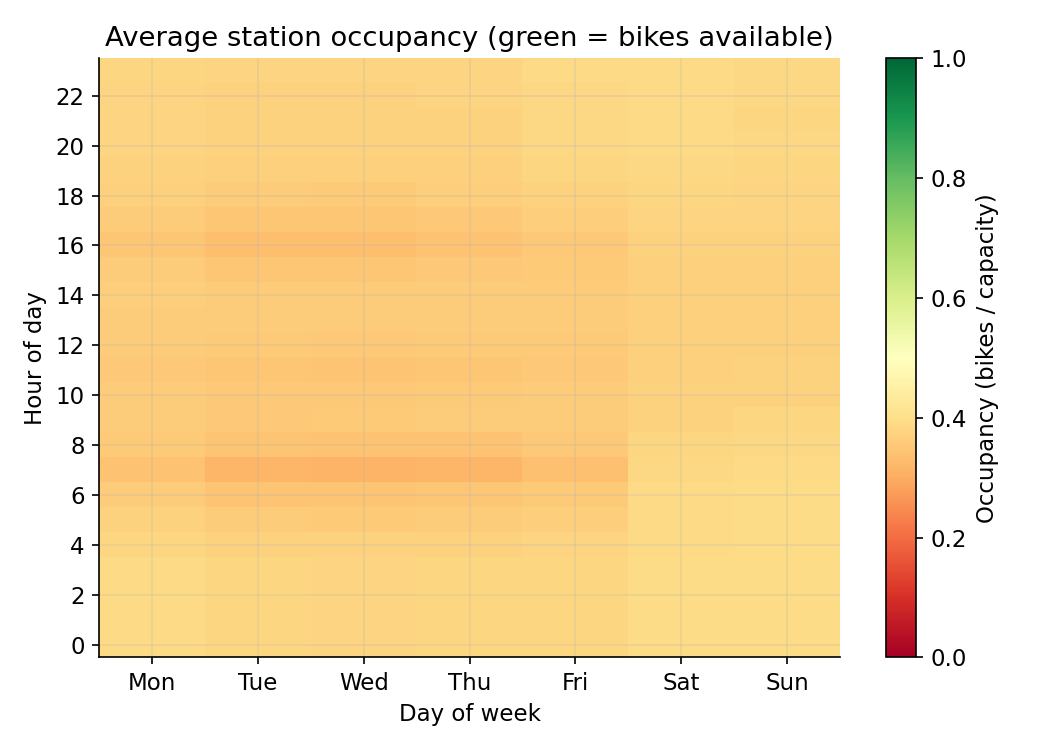
\includegraphics[width=\columnwidth]{figures/eda_occupancy_heatmap.png}}
\caption{Mean station occupancy by hour of day and day of week across all 115 stations. The weekday commuter tide is clearly visible; weekends are flat.}
\label{fig:heatmap}
\end{figure}

\subsection{Feature Representation}
Each station-hour is represented by station identity, hour of day and day of week, all one-hot encoded (147 columns after encoding), plus standardised station capacity. Hour and day are treated as categorical rather than numeric so that the linear baseline can express non-monotonic daily rhythms just as flexibly as the tree models, making the model comparison a fair contest of capacity rather than of encoding. No weather or event data are used; restricting inputs to the open feed keeps the system deployable with zero external dependencies, and the consequences of this choice are examined honestly in the discussion.

\subsection{Models}
Four approaches of increasing capacity are compared. The \textbf{naive baseline} predicts the historical mean of the target for the same station, day of week and hour over the training months, falling back to the global mean for unseen combinations; any learned model must beat this lookup table to justify its complexity. \textbf{Linear regression} fits ordinary least squares on the encoded features. The \textbf{random forest} \cite{probst2019hyperparameters} uses 200 trees with a minimum of three samples per leaf. \textbf{XGBoost} \cite{chen2016xgboost} uses 500 boosted trees of maximum depth 7 with learning rate 0.05 and subsampling of 0.9. All models are wrapped in identical scikit-learn pipelines so that encoding and scaling are fitted on training data only. Predictions are clipped below at zero, since negative bike counts are meaningless.

\subsection{Evaluation Protocol}
Evaluation is strictly temporal: models are fitted on April and May and assessed once on the entirely unseen month of June. A random split would leak each station's June regime into training and inflate every score; the temporal split mirrors real deployment, in which the model always predicts a future it has never observed. Regression quality is reported as mean absolute error (MAE), root mean squared error (RMSE) and the coefficient of determination (R squared), all in bikes. The business layer is evaluated separately: a station-hour is labelled empty-risk when actual availability is at or below two bikes, an alert fires when predicted availability is at or below the same threshold, and precision, recall and F1 are computed over all 81,588 test station-hours.

\section{Implementation and Application}
The system comprises three Python components. A \textbf{data loader} converts raw monthly files into the hourly modelling table and is shared by every downstream component, eliminating train-serve skew. A \textbf{training script} fits and evaluates all models, exports metrics, figures, the fitted best model and small precomputed prediction grids. An \textbf{analytics script} derives per-station statistics used by the application layer, including a commuter-role classification: comparing each station's mean weekday occupancy in the morning peak (07:00--09:00) against the evening peak (16:00--19:00) labels it a commuter destination (fills in the morning), a commuter origin (fills in the evening) or balanced.

The application layer is an interactive Streamlit dashboard that consumes only the precomputed outputs, so it starts instantly and never loads the heavy fitted model. It offers five views: an operations map of predicted availability, alert status or station role for any day-hour combination; a rebalancing planner; a station explorer with per-station profiles and reliability statistics; city-pattern analytics; and a model-performance page that exposes every evaluation number reported here, including the confusion matrix, so that the tool never overstates its own reliability. The planner converts the selected hour's predictions into action: stations are held to a comfort band of 25 to 75 percent occupancy, deficits and surpluses are computed against the band, and a greedy nearest-surplus pairing (haversine distance) emits a concrete move list. For the Wednesday 08:00 scenario, the planner proposes moving 26 bikes across a 27.1 km route to relieve the 49 stations predicted below their band.

\section{Results and Discussion}
\subsection{Quantitative Results}
Table~\ref{tab:results} and Fig.~\ref{fig:comparison} report held-out June performance.

\begin{table}[htbp]
\caption{Held-Out Performance, June 2026 (81,588 Station-Hours)}
\begin{center}
\begin{tabular}{lccc}
\hline
\textbf{Model} & \textbf{MAE} & \textbf{RMSE} & \textbf{R\textsuperscript{2}} \\
\hline
Naive station-day-hour mean & 4.964 & 6.579 & 0.555 \\
Linear regression & 6.595 & 8.294 & 0.293 \\
Random forest & \textbf{4.964} & \textbf{6.577} & \textbf{0.555} \\
XGBoost & 5.969 & 7.401 & 0.437 \\
\hline
\end{tabular}
\label{tab:results}
\end{center}
\end{table}

\begin{figure}[htbp]
\centerline{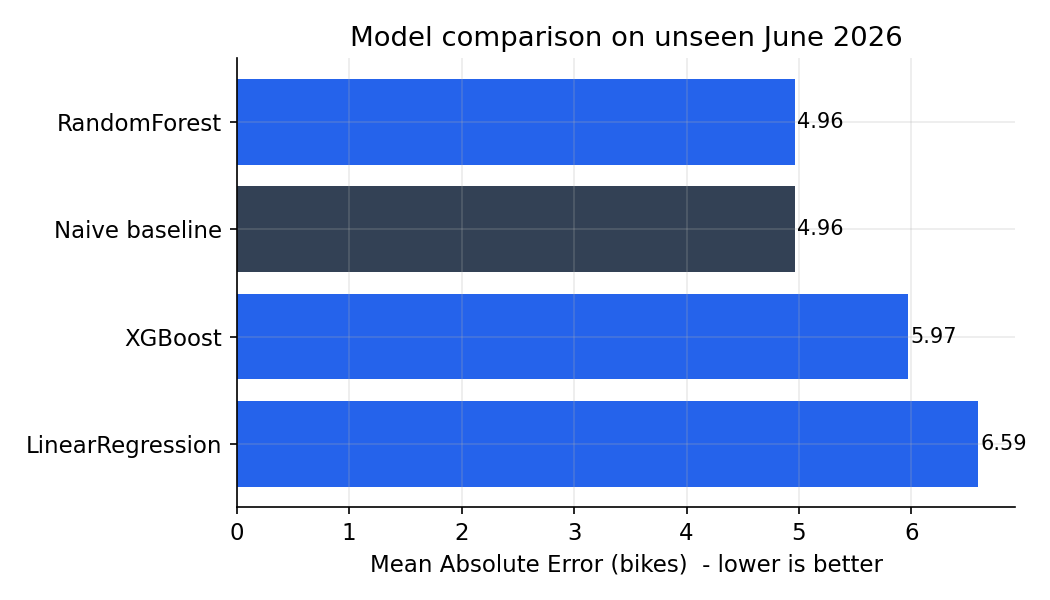
\includegraphics[width=\columnwidth]{figures/model_comparison.png}}
\caption{Model comparison on the unseen June 2026 month. The random forest and the naive baseline are separated by less than 0.001 bikes of MAE.}
\label{fig:comparison}
\end{figure}

The random forest is the best deployable model, wrong by 4.96 bikes on average against stations whose median capacity is 30 docks, and marginally ahead of the baseline on RMSE. Linear regression, despite receiving the same one-hot calendar encoding, cannot represent the interaction that matters, namely that the \emph{shape} of the daily curve differs per station, and lands 33 percent worse. XGBoost at depth 7 underfits the 147-column one-hot space relative to the forest's fully grown trees.

The most instructive result, however, is the near-tie between the random forest and the lookup-table baseline. With inputs restricted to station identity and calendar position, the weekly rhythm itself carries close to all of the predictable structure, and the forest's contribution is to match that ceiling while additionally smoothing across sparse station-hour cells and generalising to unseen combinations. This is reported as a finding rather than hidden: it quantifies exactly how far calendar features alone can go, and it defines the bar that any richer model must clear. Fig.~\ref{fig:profile} illustrates the fitted behaviour at the station with the largest daily swing, where the forest tracks the sharp morning drain closely.

\begin{figure}[htbp]
\centerline{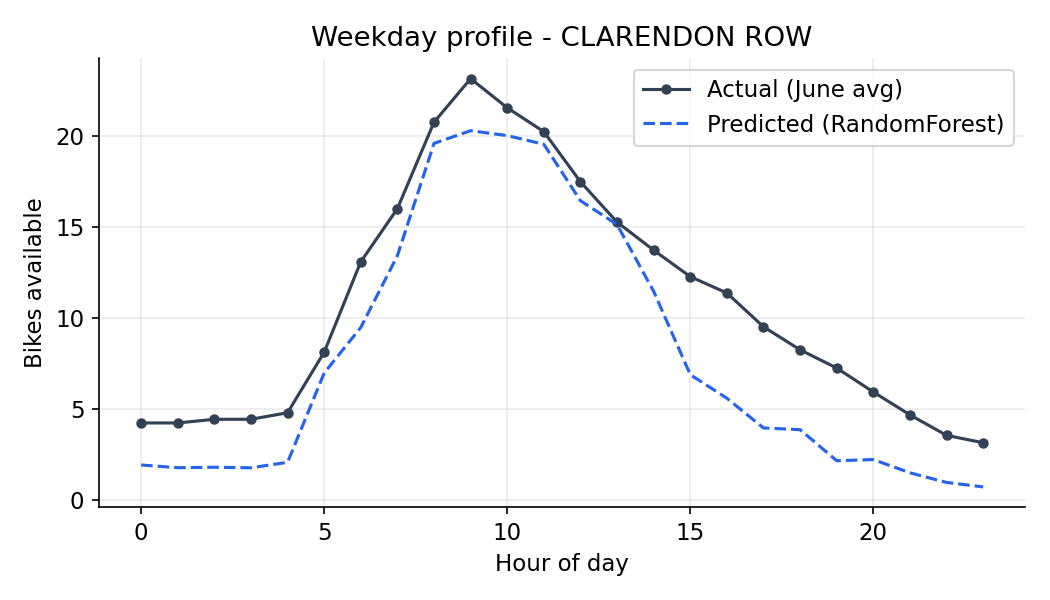
\includegraphics[width=\columnwidth]{figures/station_profile.png}}
\caption{Typical weekday profile at the highest-swing station: June actual availability versus the random forest prediction.}
\label{fig:profile}
\end{figure}

\subsection{When the Model Fails}
Fig.~\ref{fig:errhour} decomposes test error by hour. Error peaks precisely at the two commuter shoulders, around 08:00 and 17:00--18:00, when availability changes fastest and a one-hour cell mixes pre-rush and post-rush states. Operationally this is the least damaging possible failure profile: the \emph{direction} of the tide at those hours is stable and correctly predicted, and rebalancing decisions hinge on that direction more than on exact counts. Fig.~\ref{fig:importance} confirms that station identity dominates the learned importance, followed by hour of day; capacity contributes little once identity is known, as capacity is itself a fixed property of the station.

\begin{figure}[htbp]
\centerline{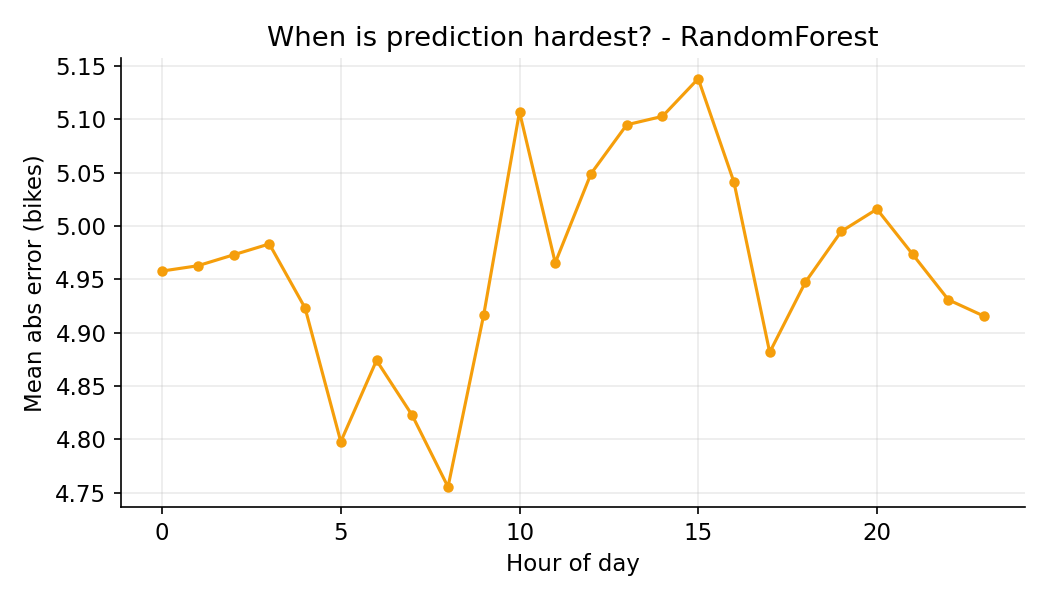
\includegraphics[width=\columnwidth]{figures/error_by_hour.png}}
\caption{Mean absolute error of the random forest by hour of day on the June test month. Errors concentrate at the morning and evening rush shoulders.}
\label{fig:errhour}
\end{figure}

\begin{figure}[htbp]
\centerline{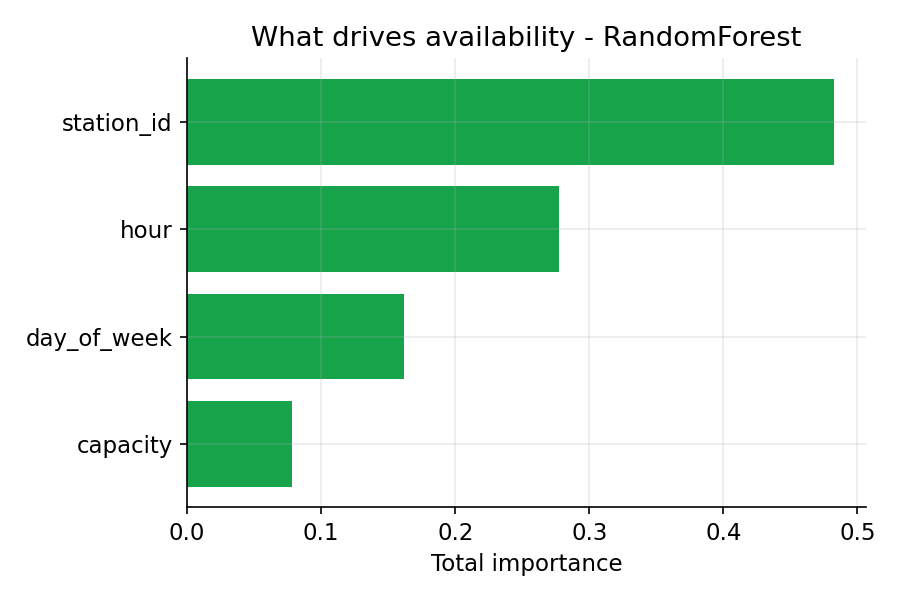
\includegraphics[width=\columnwidth]{figures/feature_importance.png}}
\caption{Grouped feature importance of the random forest. One-hot importances are summed back to their parent feature.}
\label{fig:importance}
\end{figure}

\subsection{Operational Findings}
On the business layer, 21.5 percent of June station-hours were genuinely empty-risk. The random forest's alerts achieve precision 0.776, recall 0.280 and F1 0.411 (62,611 true negatives, 1,414 false positives, 12,651 false negatives, 4,912 true positives). The system is thus tuned conservative: when it dispatches a crew it is right roughly four times in five, at the cost of catching only the most predictable 28 percent of outages, those driven by the recurring commuter pattern rather than by day-specific shocks. The dashboard exposes the alert threshold as an operational lever so that a manager can trade recall against crew workload explicitly.

The role classification yields a clean spatial story: 50 stations are commuter origins (refilling toward evening), 34 are commuter destinations (filling by morning) and 31 are balanced, and the two commuter classes separate geographically into residential rim and employment core. Combined with the per-station reliability statistics (the worst station spends 23 percent of all hours empty), this gives planners a capacity-investment map that is independent of any single day's forecast.

\section{Ethical Concerns}
The station feed contains no personal data, no trips, no accounts, no locations of individuals, only aggregate counts at fixed public infrastructure, so classical privacy risk is minimal; this is a deliberate design choice of the project. The ethical weight instead sits in how predictions steer physical service. First, spatial equity: a planner that optimises against predicted demand will concentrate service where demand is already served, and peripheral or deprived areas with chronically empty stations could be further de-prioritised, compounding transport inequality. The role and reliability views exist partly to make such chronic under-service visible rather than optimised away. Second, the precision-recall trade-off is an ethical choice disguised as a tuning parameter: a precision-tuned system quietly accepts 72 percent of outages unaddressed, and the affected riders are not randomly distributed. Third, transparency: all data, code and metrics are open and reproducible, and the dashboard surfaces the model's own confusion matrix, so the system's limits are inspectable by the public that funds the scheme. Finally, the environmental cost of the intervention itself, diesel rebalancing trucks, argues for exactly the routing-efficiency features the planner provides.

\section{Conclusion and Future Work}
This project demonstrates that a fully open, fully reproducible pipeline, three months of public dublinbikes data, classical models and honest temporal evaluation, is sufficient to forecast station availability to within five bikes and to drive concrete, high-precision rebalancing actions through an interactive operations tool. The near-tie between the random forest and the historical-mean baseline is presented as a substantive finding: calendar structure is the dominant predictable signal at the hourly horizon, and reporting that ceiling honestly is more valuable than overstating model sophistication.

Future work follows directly from the observed failure modes. Weather covariates and lagged availability (the state one and two hours earlier) target exactly the rush-shoulder errors where the calendar model is weakest; a probabilistic formulation would let alerts carry calibrated confidence; and coupling the planner's move list to a time-windowed vehicle-routing optimiser such as that of Lu and Chuang \cite{lu2024heuristic} would close the loop from prediction to dispatch.

\bibliographystyle{IEEEtran}
\bibliography{DM}

\end{document}
